\section{Benchmarks}

We evaluated the performance of GEODE on a 24-node cluster of Raspberry Pi 3 B+ single-board computers (1.4GHz 64-bit quad-core ARMv8 CPU, 1 GB RAM, 
802.11n Wireless LAN, 64 GB microSD storage) running Arch Linux ARM, Kernel 4.19. GEODE C language binaries were produced with all \texttt{gcc} compiler optimizations enabled, and the comparison with Java-based Geoavailability Grids was carried out using OpenJDK 11.0.3.

Notably, the Java VM used for benchmarking had a substantial influence on the results. Our first evaluation of Geoavailability Grids targeted OpenJDK 8, which did not support platform-specific optimizations and ran in a fully-interpreted mode. This yielded run times of over eight minutes for a single iteration of our insertion benchmark. Oracle JDK 8 provides platform-specific optimizations on our test hardware, but its garbage collector is single-threaded by default. Ultimately, we used the latest version of OpenJDK 11 for the benchmarks because parallel garbage collection was supported in addition to platform-specific optimizations.

\subsection{Insertion}

To measure data ingestion performance, we compared the insertion throughput and memory usage of GEODE with the Geoavailability Grid implementation provided in Galileo \cite{malensek2013polygon}. This included the following benchmarks:

\begin{description}
\item[NOAA One Pass:] Inserting a single point for the locations of each station in our NOAA dataset (262,792 unique locations).
\item[NOAA Two Pass:] Repeating the single pass benchmark with a second pass to measure the overhead associated with deserializing messages and converting to index coordinates; the second pass includes the same 262,792 locations and will not cause any changes to the underlying bitmaps.
\item[Random Location:] Entries in observational data streams generally do not exhibit predictable ordering or insertion sequences; this benchmark involved choosing random $(x, y)$ coordinates from a uniform distribution and inserting them into the index.
\end{description}

To establish a baseline performance measure for these benchmarks, additional features beyond the geospatial locations were not stored in memory or on disk.

Figure~\ref{fig:insert} demonstrates insertion throughput, measured by the number of records inserted per second into both index types on a single cluster node. Results were averaged over 100 iterations executed across the entire cluster. Here, GEODE assimilated records approximately 6, 4, and 418 times faster than the Geoavailability Grid implementation.

The speed differential in the NOAA benchmarks can largely be explained by (1) optimizations in converting latitude and longitude to $(x, y)$ grid points, (2) a reduction in the amount of memory allocations performed per insertion, and (3) the Roaring Bitmaps used to manage grid cells are demonstrably faster than the EWAH-based bitmaps in Geoavailability Grids \cite{lemire2016consistently}. The randomized benchmark exhibited a much greater performance differential; while the explanations listed previously for the first two benchmarks do contribute to this disparity, the most significant difference in the two approaches is their underlying bitmap implementations. The Roaring Bitmap-based grids in GEODE allow random insertions, while the EWAH-based bitmaps in Geoavailability Grids require in-order insertions. To compensate for this, random insertions into GeoGrids are batched in a sorted map and flushed periodically, resulting in memory usage fluctuations and higher allocation overhead.

\begin{figure}
    \centerline{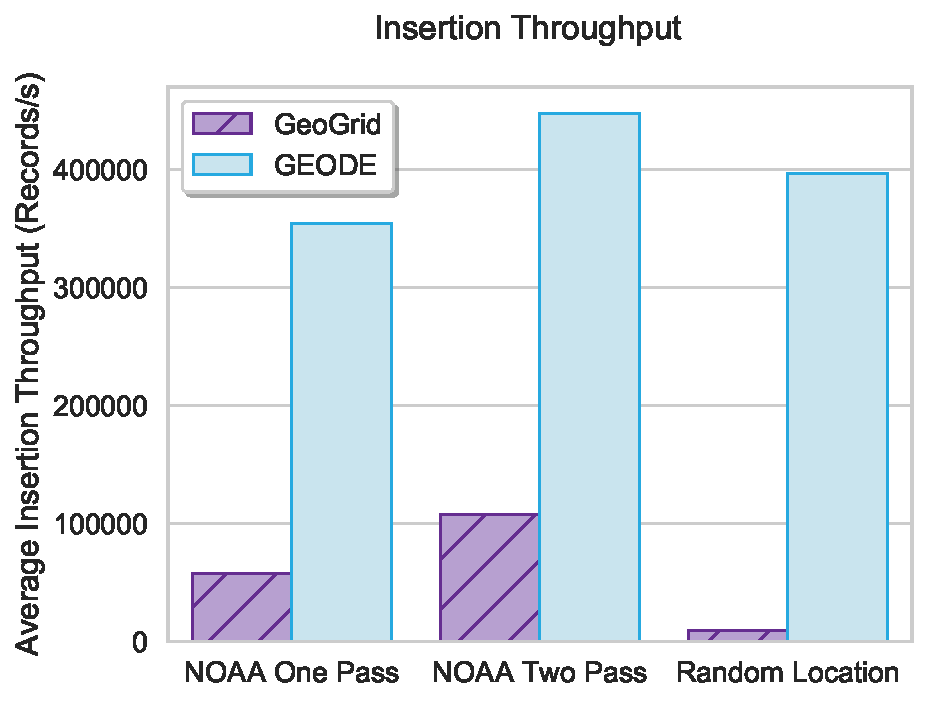
\includegraphics[width=\linewidth]{insert.pdf}}
    \caption{Insertion throughput of GEODE and Geoavailability Grids for each benchmark. Here GEODE maintains substantially higher throughputs, particularly in situations where points are inserted in random order.}
    \label{fig:insert}
\end{figure}

\begin{figure}
    \centerline{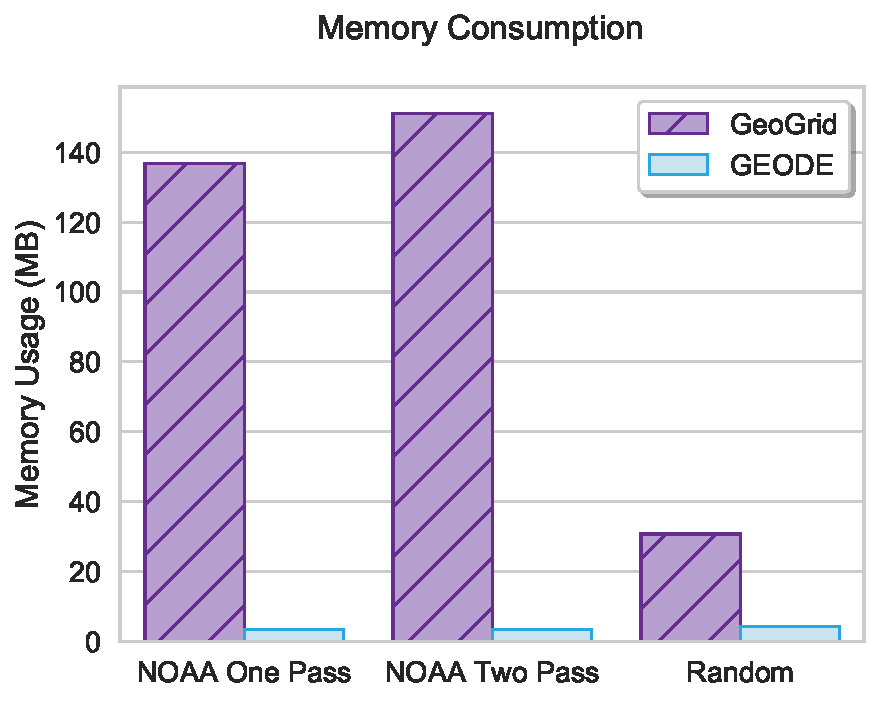
\includegraphics[width=\linewidth]{mem.pdf}}
    \caption{Memory consumed by GEODE and Geoavailability Grids for each benchmark. GEODE requires a more consistent amount of memory and fewer overall allocations.}
    \label{fig:mem}
\end{figure}

\subsection{Querying}

To measure query performance, we compared the query time of GEODE with the Geoavailability Grid implementation provided in Galileo \cite{malensek2013polygon}. This included the following benchmarks:

\begin{description}
\item[Random Location:] Entries in observational data streams generally do not exhibit predictable ordering or insertion sequences; this benchmark involved choosing random $(x, y)$ coordinates from a uniform distribution and inserting them into the index. The index was then queried with a polygon that only spans one geohash so that only one bitmap intersection is performed.
\end{description}

\begin{figure}
    \centerline{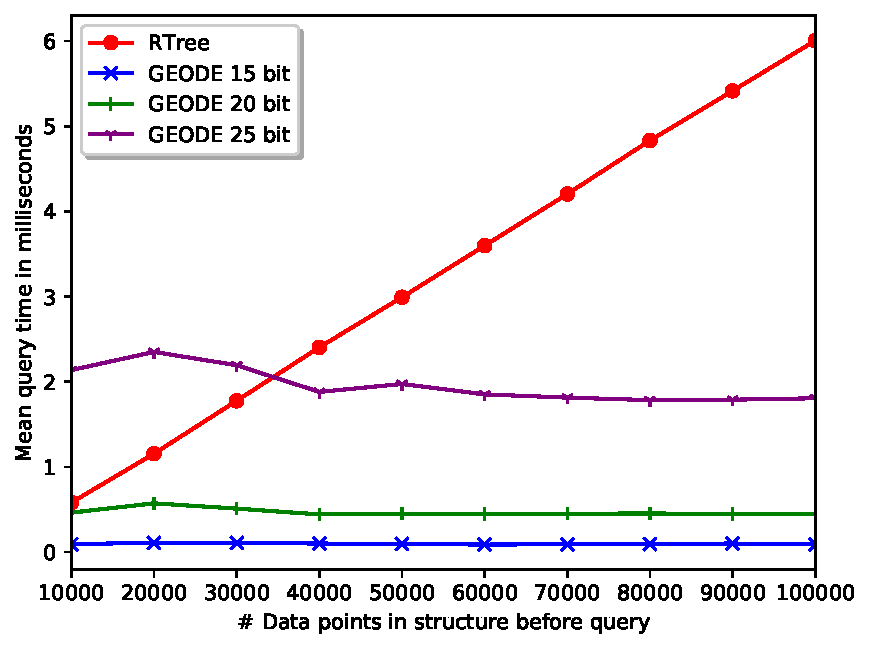
\includegraphics[width=\linewidth]{query_scatter.pdf}}
    \caption{Mean query time of GEODE and Geoavailability Grids after random insertions. GEODE has significantly better query performance compared to the rbang rtree variant, especially with larger data sets. GEODE query time stays consistent regardless of how much data is stored whereas rtree query time increases as data increases. Bitmap resolution does affect GEODE query time, but high resolution bitmaps still beat rtrees with larger datasets.}
    \label{fig:mem}
\end{figure}
